\documentclass[11pt]{article}
\usepackage[T1,T2A]{fontenc}
\usepackage[utf8]{inputenc}
\usepackage[english,russian]{babel}
\usepackage{graphicx}
\usepackage{amsmath}
\graphicspath {{img/}}

\title{\textbf{Лабораторная работа №3\\<<Исследование устройств амплитудного преобразования сигналов в системах передачи информации>>}}
\author{Перепелица А.А., ККСО-01-19}
\date{Москва, 2022 г.}
\addtolength{\topmargin}{-3cm}
\addtolength{\textheight}{3cm}
\begin{document}
\maketitle
\thispagestyle{empty}
\textbf{Цель работы:} ознакомление с устройством, работой амплитудных 
модуляторов и демодуляторов сигналов и приобретение практических навыков 
моделирования этих устройств.

\section{Схема №1: исследование АМ сигналов}
\subsection{Перечень элементов, использованных в схемах, с
их краткими характеристиками}
\begin{itemize}
    \item[-] Источник переменного тока (3.54 В, 200 Гц)
    \item[-] Четырехканальный осциллограф
    \item[-] 2 источника одночастотной амплитудной модуляции (5 В, 1000/200 Гц)
    \item[-] Анализатор спектра 
    \item[-] Ключ
\end{itemize}


\subsection{Копии окон схемных файлов с позиционными обозначениями}
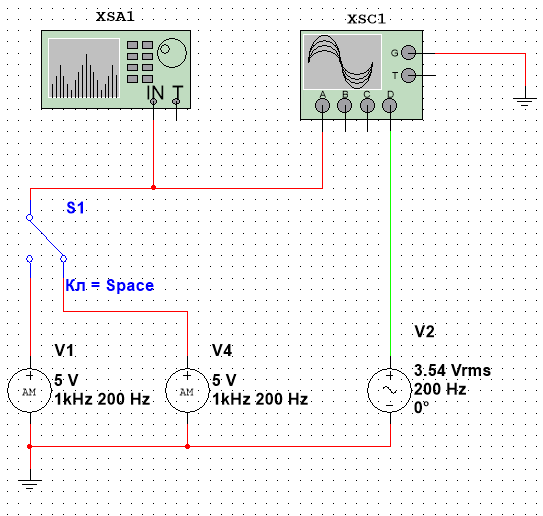
\includegraphics[width=1\linewidth]{img/first.png}
\begin{center}
    Рис.1 Схема исследования АМ сигналов
\end{center}

\subsection{Результаты расчетов и измерений приборами}
\begin{center}
    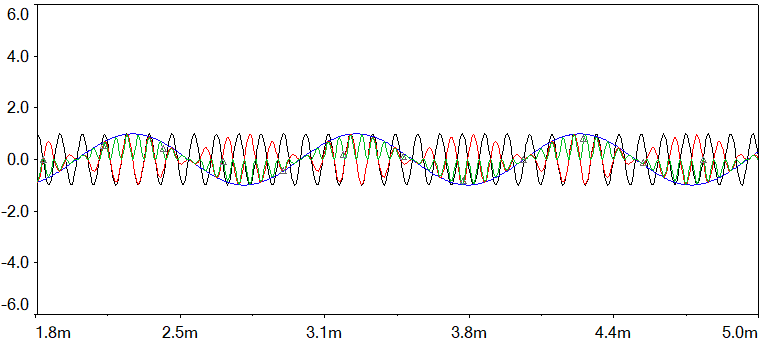
\includegraphics[width=1\linewidth]{img/second1.png}
        Рис.2 Показания осциллографа и анализатора спектра при первом положении ключа.
\end{center}

\begin{center}
    \includegraphics[width=1\linewidth]{img/second2.png}
        Рис.3 Показания осциллографа при втором положении ключа.
\end{center}

По данным показаниям можем определить коэффициент амплитудной модуляции. Вычислим этот коэффициент по второй осциллограмме:

$
M = \frac{{A_{max}+A_{min}}}{A_{max}-A_{min}} = \frac{{12.42+2.48}}{12.42-2.48}=1.4989\approx 1.5\\
$
Полученное нами значение примерно равно теоретическому значению.


\newpage
\section{Схема №2: Модель амплитудной демодуляции}
\subsection{Перечень элементов, использованных в схемах, с
их краткими характеристиками}
\begin{itemize}
    \item[-] Источник переменного тока (0.7 В, 10 кГц)
    \item[-] Четырехканальный осциллограф
    \item[-] 2 умножителя
    \item[-] Конденсатор (2мкФ)
    \item[-] Резистор (100 Ом)
\end{itemize}


\subsection{Копии окон схемных файлов с позиционными обозначениями}
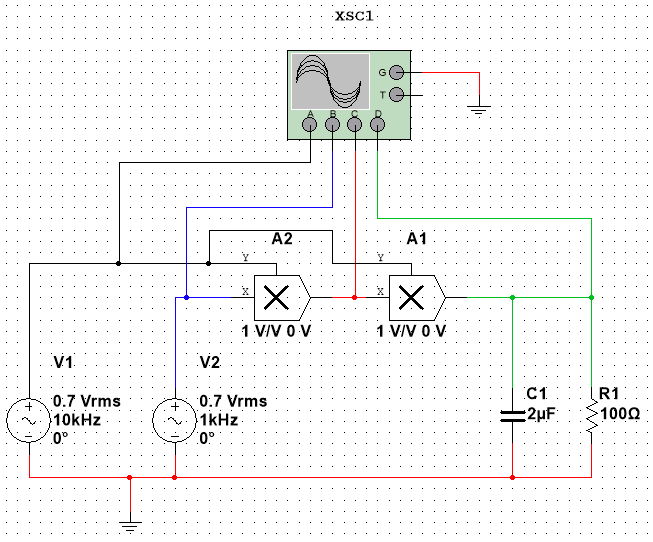
\includegraphics[width=1\linewidth]{img/second.png}
\begin{center}
    Рис.5 Схема амплитудного модулятора и демодулятора.
\end{center}

\subsection{Результаты расчетов и измерений приборами}
\begin{center}
    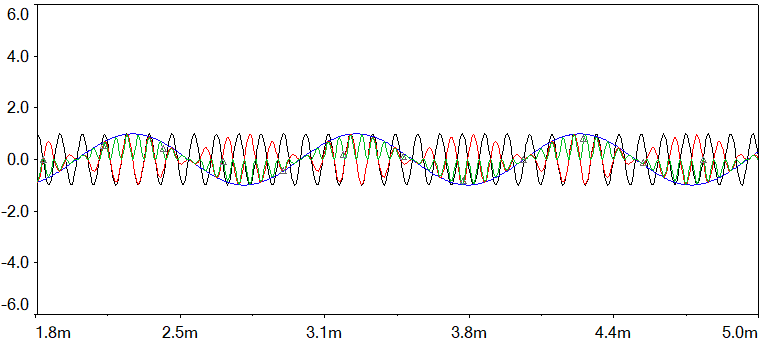
\includegraphics[width=1\linewidth]{img/second1.png}
        Рис.6 Показания осциллографа.
\end{center}
    Запаздывание выходного сигнала относительно входного:\\
    $T_2 - T_1 = 162$нС\\
    Амплитуды входного и выходного напряжений:\\
    $U_i = 6$В\\
    $U = 14$В    
\newpage
\section{ Схема №3: модель системы передачи информации с амплитудной манипуляцией}
\subsection{Перечень элементов, использованных в схемах, с
их краткими характеристиками}
\begin{itemize}    
    \item[-] Источник переменного тока (5 В, 6 Мгц)
    \item[-] Двухпроводная ЛС с потерями (50 м, 0.001 Ом)
    \item[-] Двухпроводная ЛС с потерями (25 м, 0.001 Ом) 2 шт.
    \item[-] Четырехканальный осциллограф
    \item[-] Датчик тока
\end{itemize}

\subsection{Копии окон схемных файлов с позиционными обозначениями}
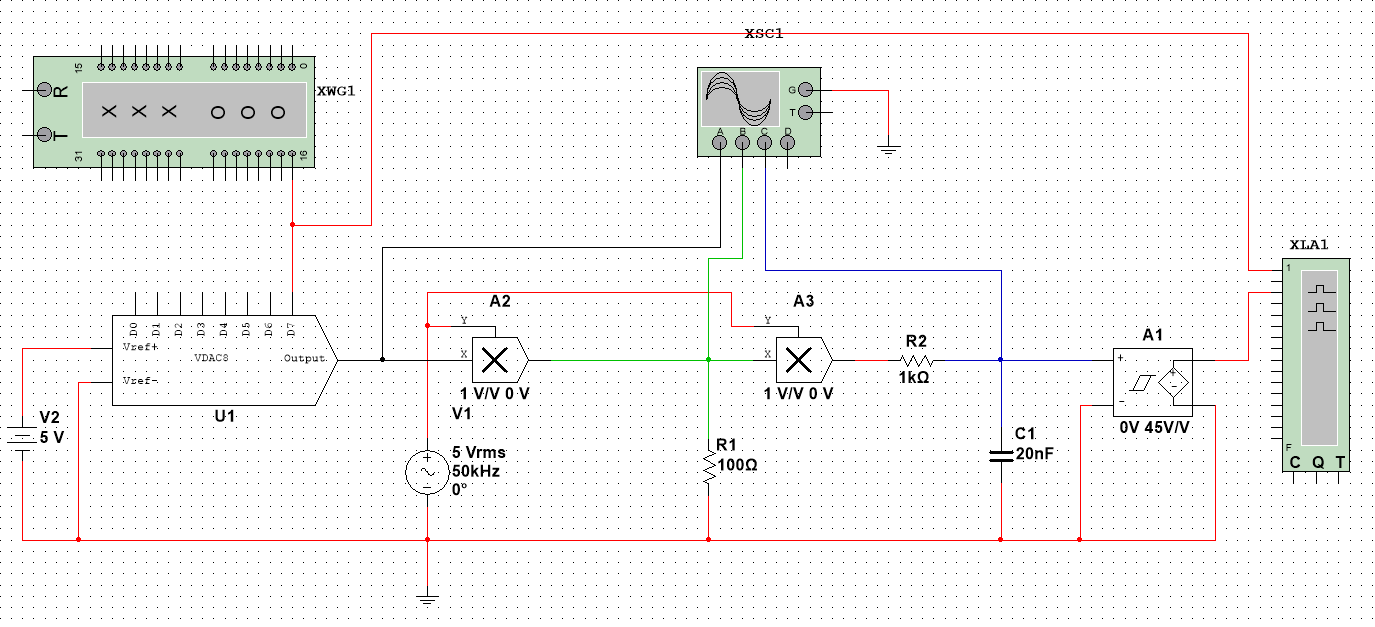
\includegraphics[width=1\linewidth]{img/third.png}
\begin{center}
    Рис.7 Схема системы передачи информации с амплитудной манипуляцией.
\end{center}

\subsection{Результаты расчетов и измерений приборами}
\begin{center}
    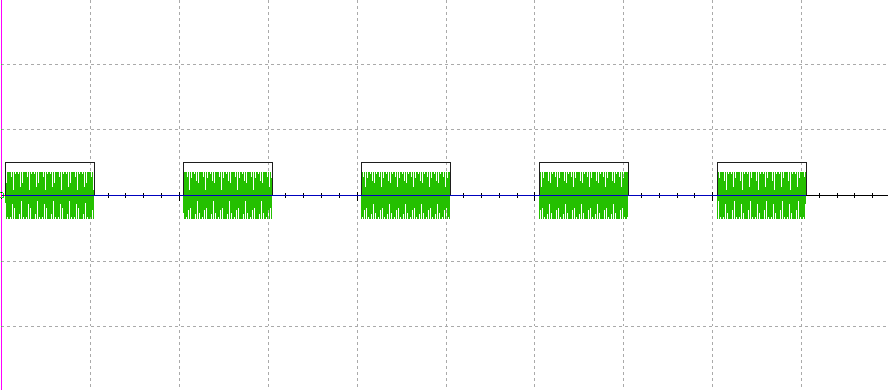
\includegraphics[width=1\linewidth]{img/third1.png}
        Рис.8 Показания осциллографа.
\end{center}


\textbf{Вывод:} в ходе выполнения лабораторной работы мы ознакомились с теорией волновых процессов в проводных линиях связи, исследовали режимы бегущих и стоячих волн.
\end{document}